\documentclass[10pt,a4paper]{article}
\usepackage[utf8]{inputenc}
\usepackage[english]{babel}
\usepackage{amsmath}
\usepackage{amsfonts}
\usepackage{amssymb}
\usepackage{makeidx}
\usepackage{graphicx}
\usepackage{fourier}
\usepackage{hyperref}
\usepackage[left=2cm,right=2cm,top=2cm,bottom=2cm]{geometry}
\author{Miguel Molinos Pérez}
\title{MPM}
\begin{document}


\title{Notes about the Generalized Interpolation Material Point
  Method} \author{
  Miguel Molinos P\'erez\\ \\
  \small{Dpto. de Matem\'aticas Aplicadas}\\
  \small{Universidad Polit\'ecnica de Madrid (UPM)}\\
  \small{\texttt{m.molinos@alumnos.upm.es}} } \date{\small{\today}}


\maketitle % Titulo
\newpage
\tableofcontents
% Idndice de contenidos

% Introduction
\include{SECTIONS/TEX/INTRODUCTION/Introduction}

% Derivation of discrete Equations
\include{SECTIONS/TEX/GOVERNING_EQUATIONS/Governing_Equations}

% The state of art of the MPM
\include{SECTIONS/TEX/MATERIAL_POINT_METHOD/Material_Point_Method}

% Explicit time integration for the mpm
\section{Explicit time integration}
\label{sec:explicit_integration}

The equation of motion presented in 

\subsection{The standard time integration scheme}
\label{sec:stand-time-integr}


\subsection{Generalized-$\alpha$ integration scheme for MPM}
\label{sec:gener-alpha-integr}

Rearranging the terms 

%%% Local Variables:
%%% mode: latex
%%% TeX-master: "../../../mpm"
%%% End:



% Stresses in the material-point method

\section{Stresses in the material-point-method}
\label{sec:stress-mater-point}

As we can see in \cite{Andersen2010}

\subsection{Objective evaluation of stresses}
\label{sec:object-eval-stress}


\subsection{Grid-crossing errors in the MPM}
\label{sec:grid-crossing-errors}

\subsection{Gravitational loading in the MPM}
\label{sec:grav-load-mpm}


\subsection{Alternative approaches for updating stresses}
\label{sec:altern-appr-updat}

The question of when to update stresses has been subjected of research
by \cite{Bardenhagen2002}. In it, Bardenhagen discusses two different
ways to update the stresses, either before or after the calculation of
internal forces. 


\subsection{Reduced integration of stress}
\label{sec:reduc-integr-stress}



%%% Local Variables:
%%% mode: latex
%%% TeX-master: "../../../mpm"
%%% End:


% Large strain formulation for the material-point-method
\include{SECTIONS/TEX/MATERIAL_POINT_METHOD/large_strain_mpm}

% Algorithms for the Material Point Method

\section{Algorithms for the Material Point Method}
\label{sec:algor-mater-point}

In this chapter, we develop several algorithms that we need for a
material point code.

\subsection{Calculus of the natural coordinates of a Gauss point}
\label{sec:calc-natur-coord}


\subsection{Local search of Gauss points}
\label{sec:local-search-gauss}

Exists several algorithms proposed by other authors to do the search
of a particle in the MPM scheme. In this case, we adopt one based on
the Gauss-Point velocity field, the

\begin{enumerate}
\item Get the list of elements that share each vertex, for this, if the
  reader is using a pointer-based programming language as C, we suggest to
  use a table of pointers in order to store the data in a more compact
  and flexible fashion. This allows also to extend this algorithm to
  any kind of mesh (IE: Quadrilaterals, triangular and hybrid). This
  step will be done at the beginning of the calculus because it is an
  information that will not change during the simulation unless we
  use some kind of automatic re-meshing algorithm.  
\item Check in first instance if the material point is in the same
  element. For this, get in first place the normal vector to the plane
  of the element with a scalar product \eqref{eq:NormaVectorElement}
  \begin{equation}
    \label{eq:NormaVectorElement}
    \overrightarrow{n} = \overrightarrow{AB} \wedge \overrightarrow{AD}
  \end{equation}
  As we can see in the figure \ref{fig:NormalVector}.
  \begin{figure}
    \centering
    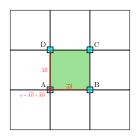
\includegraphics[scale=0.5]{./SECTIONS/TEX/ALGORITHMS/FIGURES/NormalVector}    
    \caption{Normal vector of an element}
    \label{fig:NormalVector}
  \end{figure}
  Loop over the sides of the element and check if each point satisfies
  the condition \eqref{eq:InOutSide}.
  \begin{equation}
    \label{eq:InOutSide}
    \overrightarrow{n} \cdot (\overrightarrow{AB} \wedge \overrightarrow{AP_i}) > 0
  \end{equation}
  where $\overrightarrow{n}$ is the normal vector of the element defined in
  \eqref{eq:NormaVectorElement}, $\overrightarrow{AB}$ is the array of
  the side of the element, and $\overrightarrow{AP_i}$ is the array to
  the material point measured from the initial vertex of the side. If
  it is true, for all the sides, the point is inside of the
  element, else if this condition is false in some of the sides,  the
  point it is outside and we can break the loop.  
  
  \begin{figure}
    \centering
    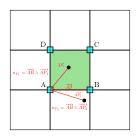
\includegraphics[scale=0.5]{./SECTIONS/TEX/ALGORITHMS/FIGURES/InOutPoint}    
    \caption{Look if the point is in our out of the element}
    \label{fig:InOutPoint}
  \end{figure}


  \item If the point is not in the same element, search in the
    neighbour elements of the initial one. In this step of the local
    algorithm, we have two chooses, the first one and the easy one to
    program is search in the elements around the initial one. The
    second one is which we have implemented in our code and consist in
    use the velocity field to predict in which element will be the
    particle. For this algorithm, this are the steps :
    \begin{enumerate}
    \item For each vertex of the element, get the direction of search
      of this vertex as the sum of the arrays of the sides that reach
      to this vertex.
      \begin{equation}
        \label{eq:VertexSeachDirection}
        \overrightarrow{n_B} = \overrightarrow{AB} + \overrightarrow{CB}
      \end{equation}
    \item For each dimension of $\overrightarrow{n_B}$, multiply it
      component by component by the velocity vector of the material
      point, like some kind of proyection, if all the components of
      the resultant vector are positive we should search the material
      point in this direction, else if try in the next node.

    \item 
    \end{enumerate}

  
  
\end{enumerate}



%%% Local Variables:
%%% mode: latex
%%% TeX-master: "../../../mpm"
%%% End:



Como vemos en \cite{Tran2019d}



% Bibliography

\bibliographystyle{acm}
\bibliography{/home/migmolper2/Documentos/PHD/BIBLIOGRAFIA/library}

\end{document}

%%% Local Variables:
%%% mode: latex
%%% TeX-master: t
%%% End:


